% Standalone TikZ flowchart
% Compile: pdflatex methodology_flowchart_tikz.tex
\documentclass[border=3pt]{standalone}
\usepackage[T1]{fontenc}
\usepackage{lmodern}
\usepackage{tikz}
\usetikzlibrary{shapes.geometric, arrows.meta, positioning, calc, shadows}

\begin{document}
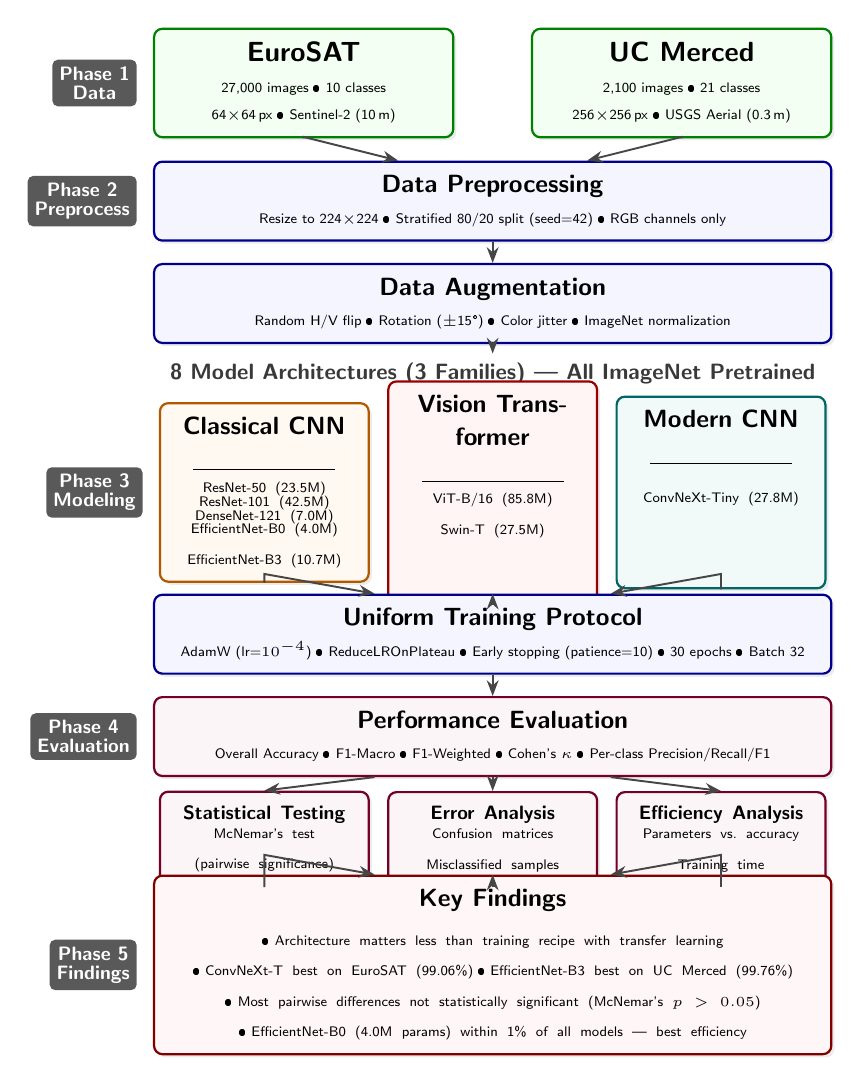
\begin{tikzpicture}[
    % Base styles
    every node/.style={font=\sffamily},
    box/.style={
        rectangle, rounded corners=3pt, line width=0.8pt,
        align=center, inner sep=5pt,
        drop shadow={shadow xshift=0.4mm, shadow yshift=-0.4mm, opacity=0.15}
    },
    % Specific styles
    dataset/.style={box, draw=green!50!black, fill=green!5, minimum width=3.8cm, minimum height=0.9cm},
    proc/.style={box, draw=blue!55!black, fill=blue!4, minimum width=8.6cm, minimum height=0.85cm},
    modbox/.style={box, minimum width=2.55cm, minimum height=2cm, text width=2.3cm},
    evalwide/.style={box, draw=purple!60!black, fill=purple!4, minimum width=8.6cm, minimum height=0.85cm},
    evalbox/.style={box, draw=purple!60!black, fill=purple!4, minimum width=2.55cm, minimum height=0.9cm, text width=2.3cm},
    finding/.style={box, draw=red!50!black, fill=red!3, minimum width=8.6cm, text width=8.2cm},
    phase/.style={
        rectangle, rounded corners=2pt, fill=gray!70!black, text=white,
        font=\sffamily\scriptsize\bfseries, align=center, inner sep=2.5pt, minimum width=1cm
    },
    arr/.style={-{Stealth[length=2mm, width=1.5mm]}, line width=0.7pt, gray!55!black},
    sectitle/.style={font=\sffamily\footnotesize\bfseries\itshape, text=gray!45!black},
]

% ============================================================
% ROW 1: DATASETS
% ============================================================
\node[dataset] (euro) at (0, 0)
    {\textbf{EuroSAT}\\[-1pt]
     {\tiny 27,000 images\;\textbullet\;10 classes}\\[-2pt]
     {\tiny 64$\times$64\,px\;\textbullet\;Sentinel-2 (10\,m)}};

\node[dataset] (ucm) at (4.8, 0)
    {\textbf{UC Merced}\\[-1pt]
     {\tiny 2,100 images\;\textbullet\;21 classes}\\[-2pt]
     {\tiny 256$\times$256\,px\;\textbullet\;USGS Aerial (0.3\,m)}};

\node[phase, left=0.2cm of euro.west, anchor=east] {Phase 1\\[-1pt]Data};

% ============================================================
% ROW 2: PREPROCESSING
% ============================================================
\node[proc] (preproc) at (2.4, -1.5)
    {\textbf{\small Data Preprocessing}\\[-1pt]
     {\tiny Resize to 224$\times$224\;\textbullet\;Stratified 80/20 split (seed=42)\;\textbullet\;RGB channels only}};

\node[phase, left=0.2cm of preproc.west, anchor=east] {Phase 2\\[-1pt]Preprocess};

\draw[arr] (euro.south) |- ([yshift=3mm]preproc.north -| euro) -- ([xshift=-1.2cm]preproc.north);
\draw[arr] (ucm.south) |- ([yshift=3mm]preproc.north -| ucm) -- ([xshift=1.2cm]preproc.north);

% ============================================================
% ROW 3: AUGMENTATION
% ============================================================
\node[proc] (aug) at (2.4, -2.8)
    {\textbf{\small Data Augmentation}\\[-1pt]
     {\tiny Random H/V flip\;\textbullet\;Rotation ($\pm$15\textdegree)\;\textbullet\;Color jitter\;\textbullet\;ImageNet normalization}};

\draw[arr] (preproc) -- (aug);

% ============================================================
% ROW 4: MODEL ARCHITECTURES
% ============================================================
\node[sectitle] (mtitle) at (2.4, -3.7)
    {8 Model Architectures (3 Families) --- All ImageNet Pretrained};

\draw[arr] (aug.south) -- (mtitle.north);

% Three model boxes - explicitly positioned to avoid overlap
\node[modbox, draw=orange!70!black, fill=orange!5] (cnn) at (-0.5, -5.2)
    {\textbf{\small Classical CNN}\\[1pt]
     {\tiny\rule{1.8cm}{0.3pt}}\\[2pt]
     {\tiny ResNet-50 (23.5M)\\[-1pt]
      ResNet-101 (42.5M)\\[-1pt]
      DenseNet-121 (7.0M)\\[-1pt]
      EfficientNet-B0 (4.0M)\\[-1pt]
      EfficientNet-B3 (10.7M)}};

\node[modbox, draw=red!60!black, fill=red!4] (vit) at (2.4, -5.2)
    {\textbf{\small Vision Transformer}\\[1pt]
     {\tiny\rule{1.8cm}{0.3pt}}\\[2pt]
     {\tiny ViT-B/16 (85.8M)\\[-1pt]
      Swin-T (27.5M)}\\[8pt]~};

\node[modbox, draw=teal!80!black, fill=teal!5] (mcnn) at (5.3, -5.2)
    {\textbf{\small Modern CNN}\\[1pt]
     {\tiny\rule{1.8cm}{0.3pt}}\\[2pt]
     {\tiny ConvNeXt-Tiny (27.8M)}\\[14pt]~};

\node[phase, left=0.2cm of cnn.west, anchor=east] {Phase 3\\[-1pt]Modeling};

% ============================================================
% ROW 5: TRAINING PROTOCOL
% ============================================================
\node[proc] (train) at (2.4, -7.0)
    {\textbf{\small Uniform Training Protocol}\\[-1pt]
     {\tiny AdamW (lr=$10^{-4}$)\;\textbullet\;ReduceLROnPlateau\;\textbullet\;Early stopping (patience=10)\;\textbullet\;30 epochs\;\textbullet\;Batch 32}};

\draw[arr] (cnn.south) |- ([yshift=2.5mm]train.north -| cnn) -- ([xshift=-1.5cm]train.north);
\draw[arr] (vit.south) -- (train.north);
\draw[arr] (mcnn.south) |- ([yshift=2.5mm]train.north -| mcnn) -- ([xshift=1.5cm]train.north);

% ============================================================
% ROW 6: PERFORMANCE EVALUATION
% ============================================================
\node[evalwide] (eval) at (2.4, -8.3)
    {\textbf{\small Performance Evaluation}\\[-1pt]
     {\tiny Overall Accuracy\;\textbullet\;F1-Macro\;\textbullet\;F1-Weighted\;\textbullet\;Cohen's $\kappa$\;\textbullet\;Per-class Precision/Recall/F1}};

\node[phase, left=0.2cm of eval.west, anchor=east] {Phase 4\\[-1pt]Evaluation};

\draw[arr] (train) -- (eval);

% ============================================================
% ROW 7: THREE ANALYSIS BOXES
% ============================================================
\node[evalbox] (stat) at (-0.5, -9.6)
    {\textbf{\scriptsize Statistical Testing}\\[1pt]
     {\tiny McNemar's test\\[-1pt](pairwise significance)}};

\node[evalbox] (err) at (2.4, -9.6)
    {\textbf{\scriptsize Error Analysis}\\[1pt]
     {\tiny Confusion matrices\\[-1pt]Misclassified samples}};

\node[evalbox] (eff) at (5.3, -9.6)
    {\textbf{\scriptsize Efficiency Analysis}\\[1pt]
     {\tiny Parameters vs.\ accuracy\\[-1pt]Training time}};

\draw[arr] ([xshift=-1.5cm]eval.south) -- (stat.north);
\draw[arr] (eval.south) -- (err.north);
\draw[arr] ([xshift=1.5cm]eval.south) -- (eff.north);

% ============================================================
% ROW 8: KEY FINDINGS
% ============================================================
\node[finding] (find) at (2.4, -11.2)
    {\textbf{\small Key Findings}\\[2pt]
     {\tiny\textbullet\;Architecture matters less than training recipe with transfer learning}\\[-1pt]
     {\tiny\textbullet\;ConvNeXt-T best on EuroSAT (99.06\%)\;\textbullet\;EfficientNet-B3 best on UC Merced (99.76\%)}\\[-1pt]
     {\tiny\textbullet\;Most pairwise differences not statistically significant (McNemar's $p > 0.05$)}\\[-1pt]
     {\tiny\textbullet\;EfficientNet-B0 (4.0M params) within 1\% of all models --- best efficiency}};

\node[phase, left=0.2cm of find.west, anchor=east] {Phase 5\\[-1pt]Findings};

\draw[arr] (stat.south) |- ([yshift=2.5mm]find.north -| stat) -- ([xshift=-1.5cm]find.north);
\draw[arr] (err.south) -- (find.north);
\draw[arr] (eff.south) |- ([yshift=2.5mm]find.north -| eff) -- ([xshift=1.5cm]find.north);

\end{tikzpicture}
\end{document}
